\documentclass{standalone}
\usepackage{graphicx}	
\usepackage{amssymb, amsmath, amsthm}
\usepackage{color}

\usepackage{tikz}
\usetikzlibrary{math, calc}

\definecolor{light}{RGB}{220, 188, 188}
\definecolor{mid}{RGB}{185, 124, 124}
\definecolor{dark}{RGB}{143, 39, 39}
\definecolor{highlight}{RGB}{180, 31, 180}
\definecolor{gray10}{gray}{0.1}
\definecolor{gray20}{gray}{0.2}
\definecolor{gray30}{gray}{0.3}
\definecolor{gray40}{gray}{0.4}
\definecolor{gray60}{gray}{0.6}
\definecolor{gray70}{gray}{0.7}
\definecolor{gray80}{gray}{0.8}
\definecolor{gray90}{gray}{0.9}
\definecolor{gray95}{gray}{0.95}
  

\begin{document}

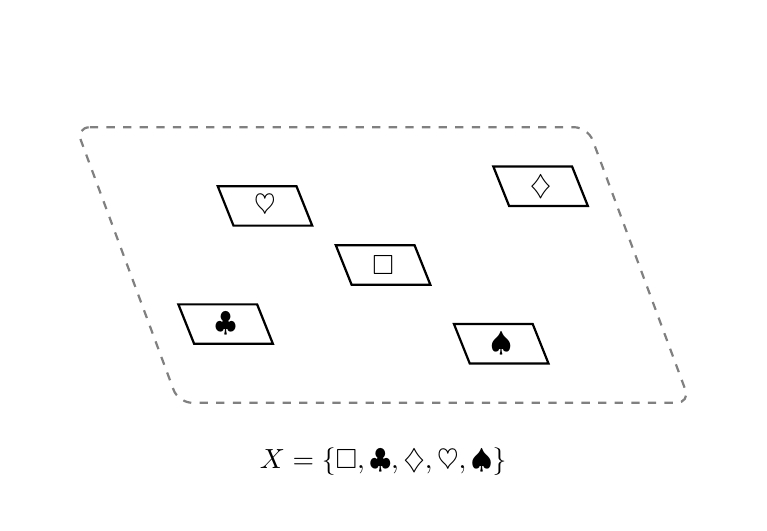
\begin{tikzpicture}[scale=1, thick]

  \draw[white] (-4.5, -3) rectangle (4.5, 3);
  
  \pgfmathsetmacro{\dx}{0.5}
  \pgfmathsetmacro{\dy}{0.25}
  \pgfmathsetmacro{\dz}{1}
  \pgfmathsetmacro{\tilt}{0.2}
  
  \foreach \x/\y\glyph [count=\n] in {0/0/\Box, -2/-0.75/\clubsuit, 2/1/\diamondsuit, 
                                      -1.5/0.75/\heartsuit, 1.5/-1/\spadesuit} {
    \begin{scope}[shift={(\x, \y)}]
      \node at (0, 0) { $\glyph$ };
      \draw[black]    ({-(1 - \tilt) * \dx}, -\dy) -- ({(1 + \tilt) * \dx}, -\dy) 
                   -- ({(1 - \tilt) * \dx}, \dy) -- ({-(1 + \tilt) * \dx}, \dy) -- cycle;
    \end{scope}
  }
  
  \draw[gray, dashed, rounded corners=5] ({-3.25 * (1 + \tilt)}, 1.75) 
                                      -- ({+3.25 * (1 - \tilt)}, 1.75)
                                      -- ({+3.25 * (1 + \tilt)}, -1.75)
                                      -- ({-3.25 * (1 - \tilt)}, -1.75) 
                                      -- cycle;
  
  \node[black] at (0, -2.5) { $X = \{ \Box, \clubsuit, \diamondsuit, \heartsuit,\spadesuit \}$ };
  
\end{tikzpicture}

\end{document}  